%
% boxmodell.tex
%
% (c) 2018 Prof Dr Andreas Müller, Hochschule Rapperswil
%
\documentclass[tikz]{standalone}
\usepackage{times}
\usepackage{amsmath}
\usepackage{txfonts}
\usepackage[utf8]{inputenc}
\usepackage{graphics}
\usetikzlibrary{arrows,intersections}
\begin{document}
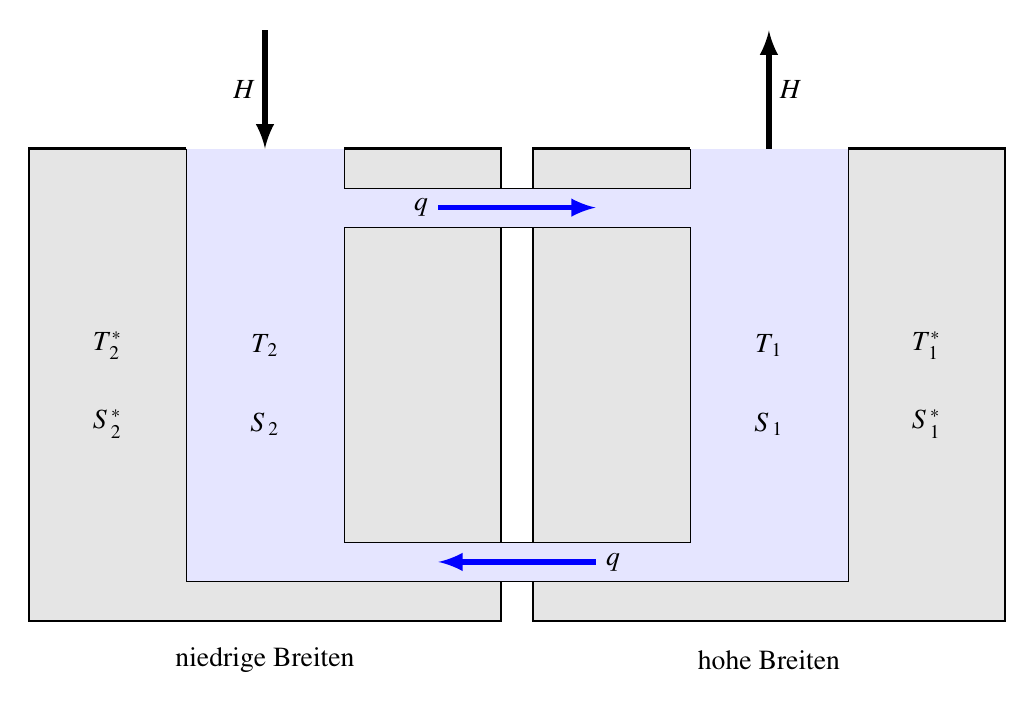
\begin{tikzpicture}[thick, >= latex, scale=1]

\def\gebiet{
\fill[color=gray!20] (-3,-3)--(3,-3)--(3,3)--(-3,3)--cycle;
\draw (-3,-3)--(3,-3)--(3,3)--(-3,3)--cycle;
\fill[color=white] (-1,-2.5)--(1,-2.5)--(1,3.1)--(-1,3.1)--cycle;
\fill[color=blue!10] (-1,-2.5)--(1,-2.5)--(1,3.0)--(-1,3.0)--cycle;
}

\begin{scope}[xshift = -3.2cm]
\gebiet
\node at (-2.0,0.5) {$T_2^*$};
\node at (-2.0,-0.5) {$S_2^*$};
\node at (0,0.5) {$T_2$};
\node at (0,-0.5) {$S_2$};
\node at (0,-3.5) {niedrige Breiten};
\draw[->,line width=2pt] (0,4.5)--(0,3);
\node at (0,3.75) [left] {$H$};
\end{scope}

\begin{scope}[xshift = 3.2cm]
\gebiet
\node at (+2.0,0.5) {$T_1^*$};
\node at (+2.0,-0.5) {$S_1^*$};
\node at (0,0.5) {$T_1$};
\node at (0,-0.5) {$S_1$};
\node at (0,-3.5) {hohe Breiten};
\draw[<-,line width=2pt] (0,4.5)--(0,3);
\node at (0,3.75) [right] {$H$};
\end{scope}

\fill[color=blue!10] (-4,-2.5)--(4,-2.5)--(4,-2)--(-4,-2)--cycle;
\fill[color=blue!10] (-4, 2.5)--(4, 2.5)--(4, 2)--(-4, 2)--cycle;

\draw[line width=0.1] (-4.2,3)--(-4.2,-2.5)--(4.2,-2.5)--(4.2,3);
\draw[line width=0.1] (-2.2,3)--(-2.2,2.5)--(2.2,2.5)--(2.2,3);
\draw[line width=0.1] (-2.2,2)--(-2.2,-2)--(2.2,-2)--(2.2,2)--cycle;

\draw[->,line width=2pt,color=blue] (1,-2.25)--(-1,-2.25);
\draw[<-,line width=2pt,color=blue] (1,2.25)--(-1,2.25);

\node at (1,-2.25) [right] {$q$};
\node at (-1,2.25) [left] {$q$};

\end{tikzpicture}
\end{document}

